
\medskip

Pour ranger les boulets de canon, les soldats du XVI\up{e} siècle utilisaient souvent un type d'empilement pyramidal à base carrée, comme le montrent les dessins suivants :

\hspace{-12mm}
\begin{tabular}{>{\centering \arraybackslash} p{2.5cm}
		>{\centering \arraybackslash} p{3.5cm}
		>{\centering \arraybackslash} p{4.5cm}
		>{\centering \arraybackslash} p{5.5cm}}
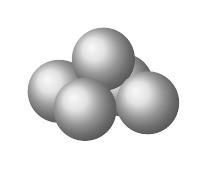
\begin{tikzpicture}[x={(6:8mm)},y=(145:4mm),z={(90:8.50mm)},baseline={(current bounding box.center)}]
\foreach \x in {2.5,3.5}{
	\shade[ball color=gray!30] (\x,3.5,1.697) circle (4mm);}
\shade[ball color=gray!30] (3,3,2.263) circle (4mm);
\foreach \x in {2.5,3.5}{
	\shade[ball color=gray!30] (\x,2.5,1.697) circle (4mm);}
\end{tikzpicture}
&
 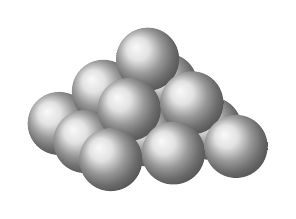
\begin{tikzpicture}[x={(6:8mm)},y=(145:4mm),z={(90:8.50mm)},baseline={(current bounding box.center)}]
\foreach \x in {2,3,4}{
	\shade[ball color=gray!30] (\x,4,1.131) circle (4mm);}
\foreach \x in {2.5,3.5}{
	\shade[ball color=gray!30] (\x,3.5,1.697) circle (4mm);}
\foreach \x in {2,3,4}{
	\shade[ball color=gray!30] (\x,3,1.131) circle (4mm);}
\shade[ball color=gray!30] (3,3,2.263) circle (4mm);
\foreach \x in {2.5,3.5}{
	\shade[ball color=gray!30] (\x,2.5,1.697) circle (4mm);}
\foreach \x in {2,3,4}{
	\shade[ball color=gray!30] (\x,2,1.131) circle (4mm);}
\end{tikzpicture}
&
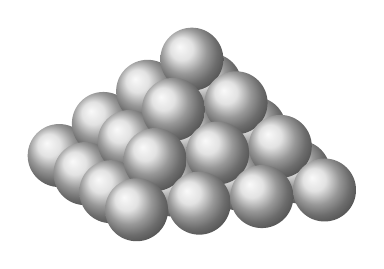
\begin{tikzpicture}[x={(6:8mm)},y=(145:4mm),z={(90:8.50mm)},baseline={(current bounding box.center)}]
\foreach \x in {1.5,2.5,...,4.5}{
	\shade[ball color=gray!30] (\x,4.5,0.5657) circle (4mm);}
\foreach \x in {2,3,4}{
	\shade[ball color=gray!30] (\x,4,1.131) circle (4mm);}
\foreach \x in {1.5,2.5,...,4.5}{
	\shade[ball color=gray!30] (\x,3.5,0.5657) circle (4mm);}
\foreach \x in {2.5,3.5}{
	\shade[ball color=gray!30] (\x,3.5,1.697) circle (4mm);}
\foreach \x in {2,3,4}{
	\shade[ball color=gray!30] (\x,3,1.131) circle (4mm);}
\shade[ball color=gray!30] (3,3,2.263) circle (4mm);
\foreach \x in {1.5,2.5,...,4.5}{
	\shade[ball color=gray!30] (\x,2.5,0.5657) circle (4mm);}
\foreach \x in {2.5,3.5}{
	\shade[ball color=gray!30] (\x,2.5,1.697) circle (4mm);}
\foreach \x in {2,3,4}{
	\shade[ball color=gray!30] (\x,2,1.131) circle (4mm);}
\foreach \x in {1.5,2.5,...,4.5}{
	\shade[ball color=gray!30] (\x,1.5,0.5657) circle (4mm);}
\end{tikzpicture}
&
 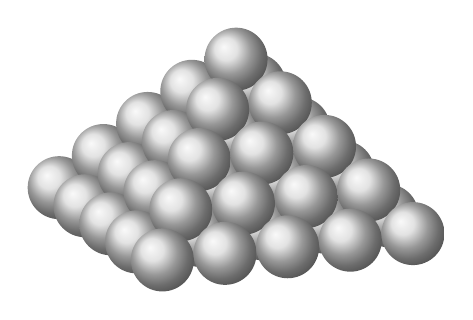
\begin{tikzpicture}[x={(6:8mm)},y=(145:4mm),z={(90:8.50mm)},baseline={(current bounding box.center)}]
 \foreach \x in {1,...,5}{
 	\shade[ball color=gray!30] (\x,5,0) circle (4mm);}
 \foreach \x in {1.5,2.5,...,4.5}{
	\shade[ball color=gray!30] (\x,4.5,0.5657) circle (4mm);}
 \foreach \x in {1,...,5}{
 	\shade[ball color=gray!30] (\x,4,0) circle (4mm);}
 \foreach \x in {2,3,4}{
	\shade[ball color=gray!30] (\x,4,1.131) circle (4mm);}
 \foreach \x in {1.5,2.5,...,4.5}{
	\shade[ball color=gray!30] (\x,3.5,0.5657) circle (4mm);}
 \foreach \x in {2.5,3.5}{
	\shade[ball color=gray!30] (\x,3.5,1.697) circle (4mm);}
 \foreach \x in {1,...,5}{
	\shade[ball color=gray!30] (\x,3,0) circle (4mm);}
 \foreach \x in {2,3,4}{
	\shade[ball color=gray!30] (\x,3,1.131) circle (4mm);}
	\shade[ball color=gray!30] (3,3,2.263) circle (4mm);
 \foreach \x in {1.5,2.5,...,4.5}{
	\shade[ball color=gray!30] (\x,2.5,0.5657) circle (4mm);}
 \foreach \x in {2.5,3.5}{
	\shade[ball color=gray!30] (\x,2.5,1.697) circle (4mm);}
 \foreach \x in {1,...,5}{
	\shade[ball color=gray!30] (\x,2,0) circle (4mm);}
 \foreach \x in {2,3,4}{
	\shade[ball color=gray!30] (\x,2,1.131) circle (4mm);}
 \foreach \x in {1.5,2.5,...,4.5}{
	\shade[ball color=gray!30] (\x,1.5,0.5657) circle (4mm);}
  \foreach \x in {1,...,5}{
 	\shade[ball color=gray!30] (\x,1,0) circle (4mm);}
 \end{tikzpicture}\\ [1.8cm]
 Empilement \linebreak à 2 niveaux&Empilement à 3 niveaux&
 Empilement à 4 niveaux&Empilement à 5 niveaux
\end{tabular}

\begin{enumerate}
	\item Combien de boulets contient l'empilement à 2 niveaux ?	
	\item Expliquer pourquoi l'empilement à 3 niveaux contient 14 boulets.	
	\item On range 55 boulets de canon selon cette méthode. Combien de niveaux comporte alors l'empilement obtenu ?	
	\item Ces boulets sont en fonte; la masse volumique de cette fonte est de \np[kg/m^3]{7300}.
	
On modélise un boulet de canon par une boule de rayon \np[cm]{6}.
	
Montrer que l'empilement à 3 niveaux de ces boulets pèse \np[kg]{92}, au kg près.
	
\emph{Rappels:}
\begin{itemize}
		\item $\emph{volume d'une boule} = \dfrac{4}{3}\times \pi \times \text{\emph{rayon}} \times \text{\emph{rayon}} \times \text{\emph{rayon}}$.	
		\item une masse volumique de \np[kg/m^3]{7300} signifie que \np[m^3]{1} pèse \np[kg]{7300}.
\end{itemize}
\end{enumerate}
 
\vspace{0,5cm}

